
\documentclass{report} 
\usepackage{amsmath}
\usepackage{amsfonts}
\usepackage{tikz}

\begin{document} 


\chapter*{Direct Monocular Articulated Visual Odometry}
\section*{Direct Monocular Visual Odometry}
We want to solve this problem: given a current camera image, previous camera
image a known camera intrinsic matrix, and a guess of the previous
depth image, derive the most likely camera motion between the current and
previous images (Fig. \ref{fig:monocular}).
Direct monocular visual odometry solves this by reprojecting all the points from
the previous camera frame into the current camera frame, and comparing the
resulting pixel intensities. That is, we want to minimize:

\begin{align}
E(\xi) &= \sum_{i}\left[I_{t - 1}(p_i) - I_t(\omega(p_i, D_{t - 1}(p_i),
\xi)\right]^2 \\
&= \sum_{i} r_i(\xi)
\label{eqn:minimization}
\end{align}
 
\noindent where $p_i \in \mathbb{R}^2$ is an image point, $I_t, I_{t - 1}$ are
the current and previous camera images, $D_{t - 1}$ is the previous depth image, 
$\xi$ is an incremental motion in $SE(3)$, and $\omega$ is the warping function
that projects a pixel from the previous image onto the current image.
Specifically, $\omega$ is of the form

\begin{equation}
\omega(p_i, z_i, \xi) = \pi^{-1}\left((\xi \circ T_{t - 1}) \pi(p_i, z)\right)
\end{equation}

\noindent where $\pi : \mathbb{R}^2 \to \mathbb{R}^3$ is the pinhole camera
projection function of the camera, $\circ$ is a compositional operator that
applies a small motion to the previous camera pose $T_{t - 1}$.

\newcommand{\drawcamera}[4]
{
	\coordinate (a) at (#1, #2);
	\coordinate (b) at ({#1 + sin(deg(#3)* 0.5 + deg(#4)) * 3}, {#2 +
	cos(deg(#3) * 0.5 + deg(#4)) * 3});
	\coordinate (c) at ({#1 + sin(-deg(#3)* 0.5 + deg(#4)) * 3},
	{#2 + cos(-deg(#3) * 0.5 + deg(#4)) * 3});
	\draw (a) -- (b);
	\draw (a) -- (c);
	\draw [ultra thick] (b) -- (c);
}

\begin{figure}
\centering
\begin{tikzpicture}
\drawcamera{8}{1}{0.75}{-0.35}
\drawcamera{1}{1}{0.75}{0.4}
\draw[-latex, dashed, thick] (8, 1) to [out=-160, in=-20] (1, 1);
\node at (4, 0) {\large$\xi$};
\node[below, right] at (8, 1) {$T_{t - 1}$};
\node[below, left] at (1, 1) {$T_{t}$};
\draw[-latex, dotted] (6.45, 3.5) -- (5, 6);
\draw[-latex, dotted] (5, 6) -- (2.8, 3.25);
\draw[fill] (5, 6.1) circle[radius=0.1];
\node[above] at (5, 6.25) {$x_i = T_{t - 1}\pi(p_i, z_i)$};
\node[right] at (6, 4.5) {$\pi(p_i, z_i)$};
\node[left] at (3.5, 4.5){$\pi^{-1}\left(T_{t}^{-1}x_i\right)$};
\draw[-latex, thick] (6.45, 3.5) to[out=160, in=20] (2.8, 3.25);
\node[below] at (4.7, 3.7) {$\omega$};
\draw[fill] (6.45, 3.4) circle[radius=0.1];
\node[below, right] at (6.45, 3.3) {$p_i$};
\end{tikzpicture}
\caption{An image point $p_i$ is unprojected out of camera frame $T_{t - 1}$,
and then projected back onto the image of the camera at $T_{t}$. The offset in
$SE(3)$ between the camera frames is $\xi$. The warp between the image point in
frame $t - 1$ and frame $t$ is given by the function $\omega$.}
\label{fig:monocular}
\end{figure}

Equation \ref{eqn:minimization} is generally minimized using Gauss Newton, with
the update:

\newcommand{\J}{\mathbf{J}}
\newcommand{\eval}{\big|}
\begin{equation}
\Delta \xi = (\J^T\J)^{-1} \sum_{i}\left(\J_i r_i(\xi)\right)
\label{eqn:update}
\end{equation}

Now, the Gauss-Newton update contains the term $\J$, which is the partial
derivative of the stacked residuals with respect to a small motion $\xi$. It has
the form:

\begin{equation}
\J = \big[\J_1 | \ldots | \J_K\big]
\end{equation}

\noindent where each $\J_i$ is the jacobian of a particular residual with
respect to a small motion $\xi$, and has the form:

\begin{equation}
\J_i = \nabla I \eval_{\omega\left(x_i, T_t\right)} \frac{\partial \pi}{\partial
p_i}
\eval_{T_t p_i} \frac{\partial T p_i}{\partial T} \eval_{T_t} \frac{\partial T
T_t}{\partial T} \frac{\partial \text{exp}(\hat \xi)}{\partial \xi} \eval_0
\label{eqn:jacobian}
\end{equation}

Equation \label{eqn:jacobian} is quite complicated. It has 4 terms to convert
between image gradients to motion on the Lie manifold of $SE(3)$:

\begin{itemize}
  \item $\nabla I \eval_{\omega\left(x_i, T_t\right)} \in \mathbb{R}^{1 \times
  2}$ is the gradient of the image at time $t$ evaluated at the projected point.
  This is easily computed by finite-differencing the image.
  \item $\frac{\partial \pi}{\partial
p_i}
\eval_{T_t p_i}$ is the derivative of the camera's projection
function with respect to a change in the projected point from the previous
image. This can be computed in closed form.
\item $\frac{\partial T p_i}{\partial T} \eval_{T_t} \in \mathbb{R}^{3 \times
12}$ is the partial derivative of the projected image point with respect to the
current transformation. This can be directly computed.
\item $\frac{\partial T
T_t}{\partial T} \frac{\partial \text{exp}(\hat \xi)}{\partial \xi} \eval_0 \in
\mathbb{R}^{12 \times 6}$ converts a change in pose into an infinitesimal
increment on the Lie manifold. This is known in closed form, and relies on the
``exponential map'' of $SE(3)$
\end{itemize}

\noindent note that 

\begin{equation}
\frac{\partial \pi}{\partial
p_i}
\eval_{T_t p_i} = \left( \begin{array}{ccc}
f_x \frac{1}{z'} & 0 & -f_x \frac{x'}{z'^2} \\ 
0 & f_y \frac{1}{z'} & -f_y \frac{y'}{z'^2}  \end{array} \right)
\end{equation}

\noindent where $T_t p_i = (x', y', z')$, and $f_x, f_y$
come from the camera intrinsics.

Optimization then proceeds by the standard Gauss-Newton rules, with necessary
conversions between poses in $T \in SE(3)$, and increments $\xi$ along the 6DOF
Lie manifold. 

This is done (in contrast to using something like a quaternion or rotation
matrix representation for $\xi$) since it prevents degenerate solutions and
allows Gauss-Newton to proceed with exactly 6 variables.

\section*{The Articulated Case}

\begin{figure}
\centering
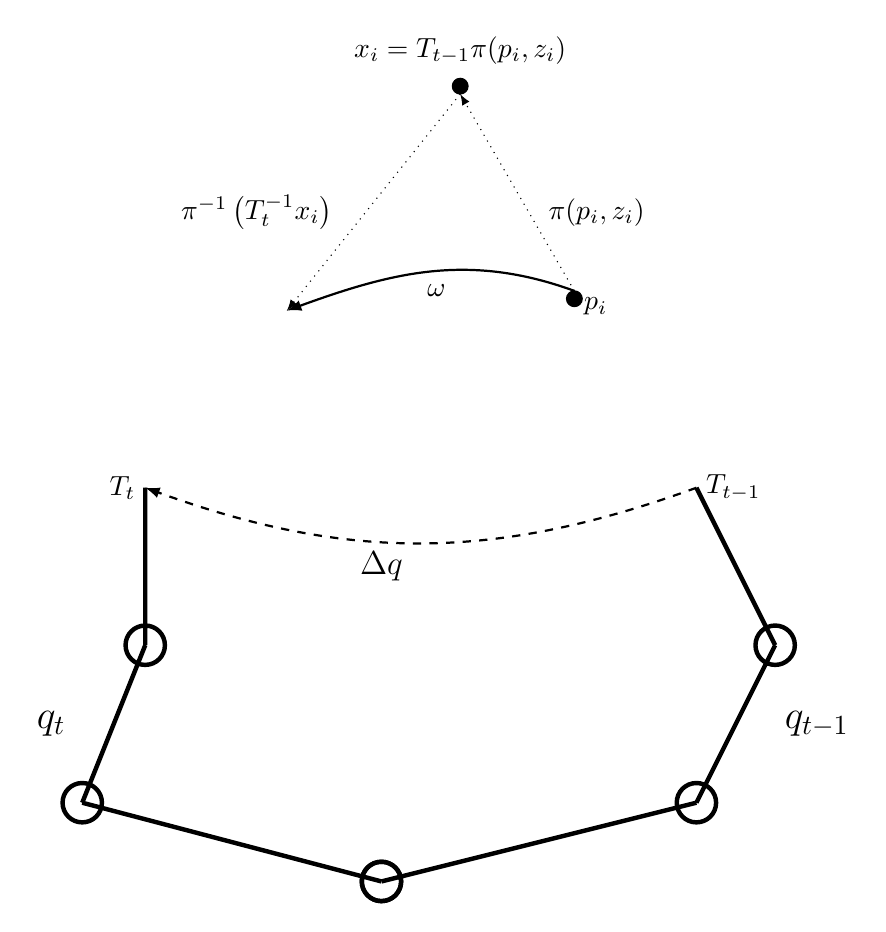
\begin{tikzpicture}
\drawcamera{8}{1}{0.75}{-0.35}
\drawcamera{1}{1}{0.75}{0.4}
\coordinate (orig) at (4, -4); 
\draw[ultra thick, line join=round] (orig) circle[radius=0.25] -- (0.2, -3)
circle[radius=0.25] -- (1, -1) circle[radius=0.25] -- (1, 1); 
\draw[ultra thick,
line join=round] (orig) circle[radius=0.25] -- (8, -3) circle[radius=0.25] --
(9, -1) circle[radius=0.25] -- (8, 1); \draw[-latex, dashed, thick] (8, 1) to
[out=-160, in=-20] (1, 1); \node at (4, 0) {\large$\Delta q$}; \node[below,
right] at (8, 1) {$T_{t - 1}$}; \node[below, left] at (1, 1) {$T_{t}$};
\draw[-latex, dotted] (6.45, 3.5) -- (5, 6);
\draw[-latex, dotted] (5, 6) -- (2.8, 3.25);
\draw[fill] (5, 6.1) circle[radius=0.1];
\node[above] at (5, 6.25) {$x_i = T_{t - 1}\pi(p_i, z_i)$};
\node[right] at (6, 4.5) {$\pi(p_i, z_i)$};
\node[left] at (3.5, 4.5){$\pi^{-1}\left(T_{t}^{-1}x_i\right)$};
\draw[-latex, thick] (6.45, 3.5) to[out=160, in=20] (2.8, 3.25);
\node[below] at (4.7, 3.7) {$\omega$};
\draw[fill] (6.45, 3.4) circle[radius=0.1];
\node[below, right] at (6.45, 3.3) {$p_i$};
\node[right] at (-0.5, -2) {\Large$q_t$};
\node[right] at (9, -2) {\Large$q_{t - 1}$};
\end{tikzpicture}
\caption{A camera mounted to a moving robot arm. The case is the same as in Fig.
\ref{fig:monocular}, except the transformation between the two camera frames is given by $\Delta q$, instead of
$\xi$, since the camera motion is constrained by the kinematics of the robot.}
\label{fig:articulated}
\end{figure}

When we don't have a free-floating camera, and instead have a camera on the end
of a constrained, articulated manipulator (Fig. \ref{fig:articulated}), the
problem is slightly different.
A robot manipulator with configuration $q \in \mathbf{R}^N$ has a forward
kinematics function $F(q) : \mathbf{R}^N \to SE(3)$ defining the pose of the
sensor. We can also write $F(q, x) : \mathbf{R}^N \times \mathbf{R}^3 \to
\mathbf{R}^3$ which transforms a point in the camera frame into the world frame
given a configuration of the robot.

In this case, the cost function we'd want to minimize is:

\begin{align}
E(\Delta q) &= \sum_{i}\left[I_{t - 1}(p_i) - I_t(\omega(p_i, D_{t - 1}(p_i),
\Delta q)\right]^2 \\
&= \sum_{i} r_i(\xi)
\label{eqn:articulated_minimization}
\end{align}

\noindent where the warping function is now:

\begin{equation}
\omega(p_i, z_i, \Delta q) = \pi^{-1}\left(F(q_{t - 1} + \Delta q, \pi(p_i,
z)\right)
\end{equation}

Notice that the $SE(3)$ compositional operator $(\circ)$ has been replaced by
simple addition. This is important, because it has removed the complicated mess
of converting between Lie manifold coordinates and transformation matrices.
Instead, we can do the whole optimization in the configuration space of the
robot, which is Euclidean. That means the Jacobian is now:

\begin{equation}
\J_i = \nabla I \eval_{\omega\left(p_i, z_i, 0\right)} \frac{\partial
\pi}{\partial p_i}
\eval_{x_i} \frac{\partial F(q, x_i)}{\partial q} \eval_{q_{t - 1}} 
\end{equation}

\noindent and it has size $N \times 1$, rather than $6 \times 1$. The
complicated Lie manifold conversions get replaced by the simple translational manipulator
Jacobian $\frac{\partial F(q, x_i)}{\partial q} \eval_{q_{t - 1}}$, evaluated
for a point projected from the previous image, which can be computed easily in
closed form.

\end{document}
